% !TEX root = ../../main.tex
\begin{figure}[H]
  \centering
  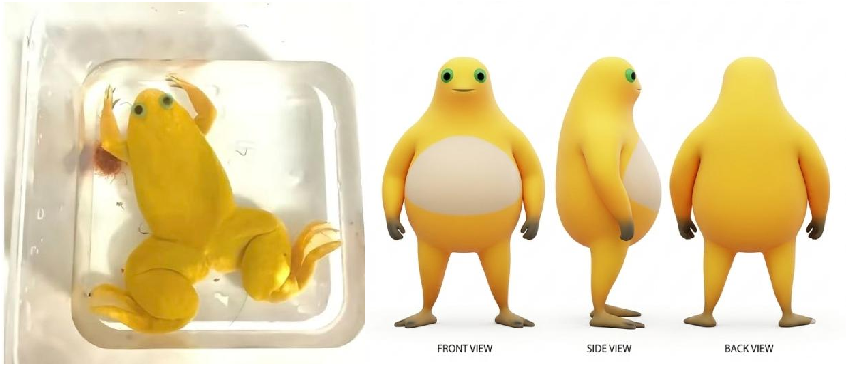
\includegraphics[width=345.61bp,height=0.76\textheight,keepaspectratio]{figures/chapter01/figure01_5.pdf}
  \renewcommand{\thefigure}{1.5}
  \caption{“现实中的奶蛙”非洲爪蟾（左）和奶蛙的三视图，后视图具有明显蛙类特征（右）}
  \label{fig:01-5}
\end{figure}
